\chapter{Implementation} \label{cha:implementation}

In this chapter, the implementation procedure of the features in \charef{cha:design} are documented, as well as the overall architecture and the choices made in regard to this. The behaviour of the robot is also described, followed by an explanation on how the implemented motor controller works.

%Finally, the finished modules of the \projname{} were listed and documented.

% Implementation procedure
\section{Implementation procedure} \label{sec:imp-procedure}

To implement the features listed in \charef{cha:design}, a stepwise approach was utilised. First, the finished design concept was cut into modules, each with a clearly defined, separate task to accomplish. These modules are what constitutes the final product, however it is possible to implement each of them independently of the others. The modules were ordered according to their importance and relevance to the final product's overall quality, and then tested and implemented in the order seen below.

\begin{enumerate}
\item Basic movement
\item Object collection
\item Bluetooth communication
\item Boundary detection
\item Object detection
\item Basic object navigation
\item Advanced movement
\item Advanced route navigation
\end{enumerate}

This approach made it possible to ensure, that a new feature or module of the robot would only be implemented, when the robot's previously implemented modules are fully operational and complete. This means that each module is known to be working correctly, the challenge is then to combine these. 

This should not be viewed as an absolute approach: work did begin on the next iterations, even if the prior ones weren't finished yet, however it serves well to illustrate how the process was planned and in what order the features were added.

To visualise these modules, a flowchart tool was used to map the different actions and considerations the robot makes when complete. Each added module of functionality was assigned with a new colour to maintain an overview of the iterations. 

\begin{figure}[H]
     \center{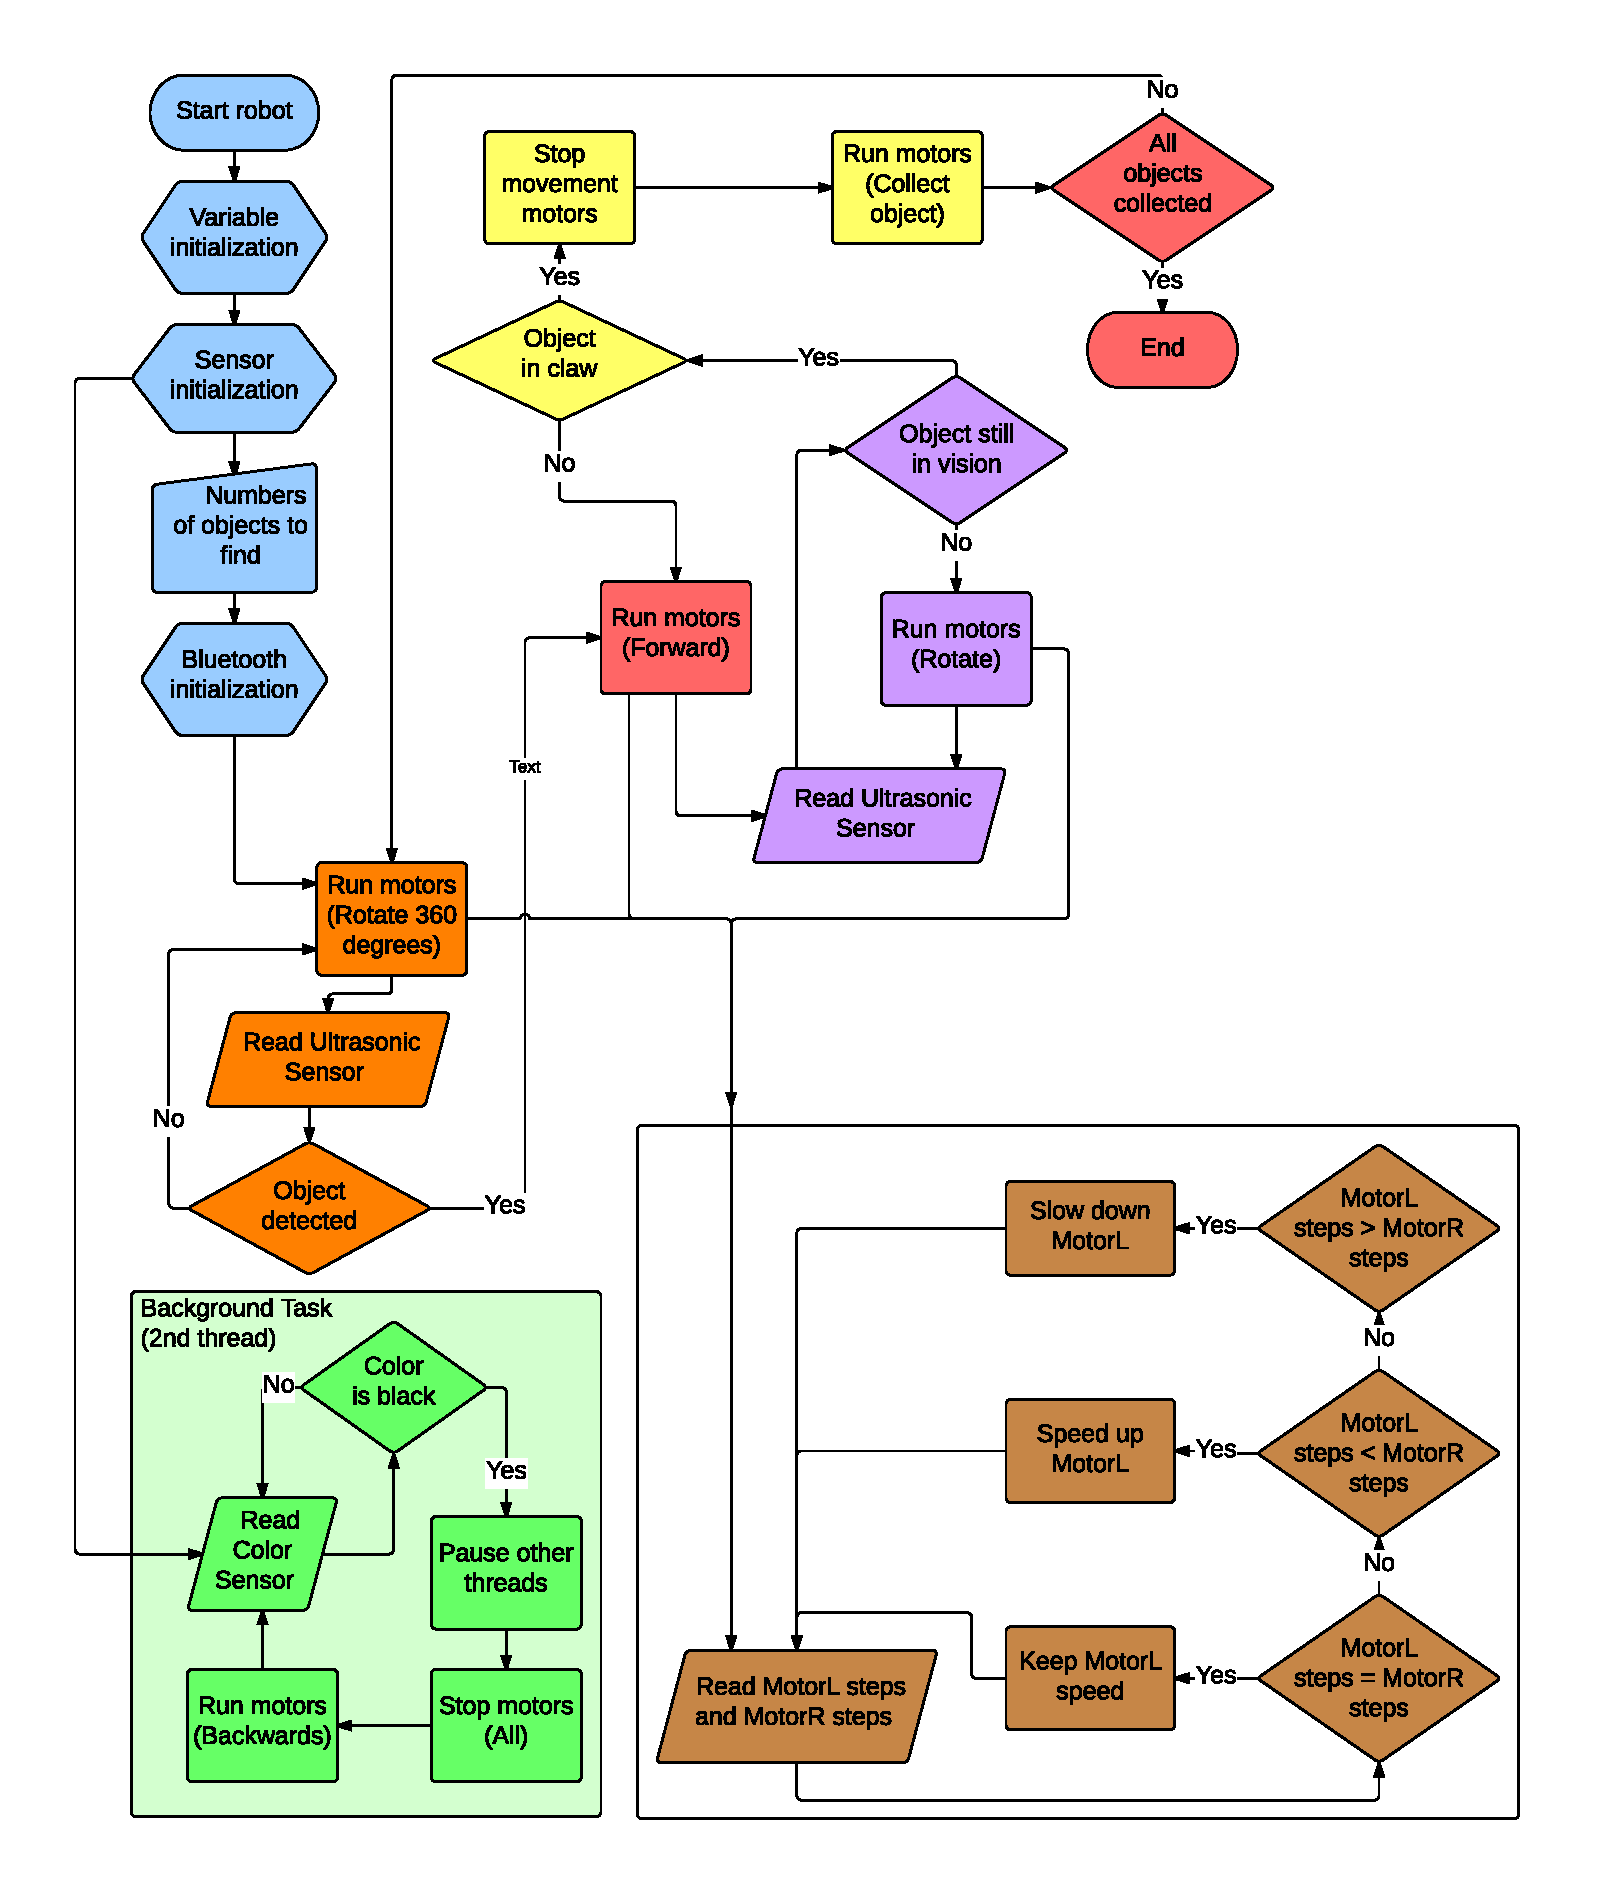
\includegraphics[width=\textwidth]
     {graphics/CompleteRobotFlowchart.pdf}}
     \caption{\label{fig:CompleteRobotFlowchart} Flowchart of the robot and its behaviour.}
\end{figure}
\fxnote{Skal vi tilføje tekst til MC boksen?}

In the diagram in \figref{fig:CompleteRobotFlowchart}, the sections are coloured according to what functionality they fulfil. The previously mentioned iterations often focus on one of the particular partitions of the flowchart. The iterations are described below.


\subsubsection{First iteration --- Basic movement}
In the first iteration, the first module was implemented: the basic movement behaviour. This iteration resulted in a basic robot with tank treads, that could move forward and backwards, and turn left and right around its own vertical axis. The robot, at this point, was able to move around in a square pattern, and end up at the starting location, with an accuracy of a few centimetres. Movement accuracy at this point was hard coded. The blue part in \figref{fig:CompleteRobotFlowchart}, which is the basis for all implementation, was also implemented in this iteration, except for the bluetooth initialisation.


\subsubsection{Second iteration --- Object collection}
In the second iteration, the robotic arm and claw used to collect objects were designed, built and developed. This collection module was tested and tweaked separately, after which it was implemented into the robot itself. This module corresponds to the yellow part in \figref{fig:CompleteRobotFlowchart}.


\subsubsection{Third iteration --- Bluetooth communication}
With the \projname{} being able to move, controlled by one of the NXT brick, and a claw and arm capable of collecting objects controlled by another brick, communication between these two bricks was the next priority to implement. This was done using the inherent Bluetooth-capabilities of the bricks. The master brick sends instructions to the slave brick, and await confirmation from the slave brick, when the task is done. This allowed for the code and behaviour to be centralised on one brick, only communicating simple instructions once in a while over Bluetooth.


\subsubsection{Fourth iteration --- Boundary detection}
This iteration implemented the colour sensors, and made it possible to detect the environment boundaries. This includes functionality to stop, reverse, and turn away from the detected line, searching for new objects. This entire feature runs in a thread by itself. This corresponds to the green part in \figref{fig:CompleteRobotFlowchart}. 


\subsubsection{Fifth iteration --- Object detection}
This iteration included the implementation of basic object detection; the \projname{} is at this point able to turn 360 degrees around while scanning for objects with the ultrasonic sensor. The ultrasonic sensor is able to detect the distance between the robot and the target object. This corresponds to some of the states in the orange part in \figref{fig:CompleteRobotFlowchart}.


\subsubsection{Sixth iteration --- Object navigation}
This iteration focused on implementing the next-in-view algorithm to find and collect objects within the boundary. The routine to find lost objects, as described in \secref{sec:niv-algorithm}, can be seen in \figref{fig:CompleteRobotFlowchart} as the purple part.


\subsubsection{Seventh iteration --- Advanced movement}
During this iteration a motor controller was developed, to ensure that the motors drive alike, in the amount of steps driven. This motor controller is used to drive straight forwards and backwards with greater precision, than the basic movement it replaces. Another motor controller was developed, but this one is used to turn the \projname{} with precision. This motor controller is used to turn a given amount of degrees, or get to a heading, choosing the most relevant turning direction. This feature is shown in the brown part in \figref{fig:CompleteRobotFlowchart}.


\subsubsection{Eight iteration --- Advanced route navigation}
The last iteration was supposed to implement the NN-algorithm described in \secref{sec:nn-algorithm}, but due to the result of the hardware test, it was decided not to implement the NN-algorithm in the final version. The ultrasonic sensor was not able to detect objects with enough precision so that the \projname{} could accurately calculate any useful information based on the data. Due to this limitation, the \emph{next-in-view} algorithm was chosen for implementation. The source code of the NN-algorithm can be found in \appref{app:CD}.


%The hardware problems, primarily the ones caused by the ultrasonic sensor, were too difficult to solve at this point in the project and this iteration will therefore not be implemented in the final program. Instead, the next-in-view algorithm will be the final algorithm. It is possible to see what would have been implemented in \secref{sec:object-navigation}. A comparison between algorithms, and a more detailed explanation of them, can be seen in \secref{sec:algorithm-desc}.

%The blue section, with the \emph{Start robot} node, is the initial start-up phase of the robot. Variables and sensors are initialised, and the number of objects to look for is determined through user input. This is the basis for the implementation. The parts marked in red describe the behaviour of the movement module. The initial implementation of the movement was the ability to move forwards, backwards and to turn left and right with some precision. The yellow part is the object collection behaviour, which handles the movement of the claw and arm that grab hold of and then collect the objects in the environment. After the arm and claw could successfully grab and collect objects, it was implemented into the movement module, to prevent the robot from changing position while an object is being collected.

%Afterwards, the purple part --- the object-detecting half of the scanning module --- was implemented, to allow the robot to actually detect the objects and determine when to activate the collection module. This module also guides the movement module's behaviour, since the movement at this stage is based on where the 

%one brick being the master unit sending instructions, the other being the slave, receiving instructions and returning confirmation. In the case of \projname{}, the brick with the scanners and the movement control was chosen to be the master, and the brick in control of the object collection module the slave. This allowed for the code and behaviour to be centralised on one brick, only communicating simple instructions once in a while over Bluetooth. 

%This iteration focus on implementing a more intelligent way to locate and collect all objects. At this point the robot is able to locate all the visible objects from the starting position. The robot turn 360 degrees and save the angle and distance of all the objects which the robot detects. The \projname{} then navigates to the spotted objects in sequence and attempts to grab these. If the boundary is spotted while driving to a object, then the \projname{} abandons the object, and moves on to the next object. 

%moving towards any object spotted. When it is within sufficient range of the object, it will attempt to pick up the object using the previously implemented collection module. This basic object detection allows the robot to --- in some cases --- complete the intended task successfully.

% Architecture 
\section{Architecture} \label{sec:architecture}
This section focuses on the architecture of the program. Firstly, tasks, events, and alarms used in the \projname{} are discussed. Then follows a number of sequence diagrams, that outlines the function of each task. 


\subsection{Tasks, events, and alarms} \label{sec:task-events-alarms}
This section focuses on the tasks, events, and alarms used in the \projname{}. These are all declared in an OSEK Implementation Language (OIL) specification. All the static declaration of system objects are specified in the OIL file. The OIL specification and the code makes up the program~\citep{nxtOSEK2}. The following subsections focuses on tasks, events, and alarms, what they are and how they are used in the \projname{}.

\subsubsection{Tasks} \label{sec:tasks}
nxtOSEK utilises task to control the program execution, where it is possible to have multiple tasks in one program. There is always a main task from which the primary code is executed. Another common task is one that ensures that certain sensors keeps doing their job. For example if the robot is equipped with colour sensors, the tasks will have to keep pinging the colour sensors which will keep them activated. This sort of task will have to follow a clock to ensure that there is always the same amount of time between each ping to the colour sensor. Each task must be declared in the OIL file. \lstref{lst:taskexample} shows an example of a task declaration, from the \projname{} project. 

\begin{lstlisting}[caption= An example of a task used in the \projname{}, label=lst:taskexample]
TASK MainTask
{
    AUTOSTART = TRUE { APPMODE = appmode1; };
    PRIORITY = 2;
    ACTIVATION = 1;
    SCHEDULE = FULL;
    STACKSIZE = 512;
    EVENT = EventMainTask;
    EVENT = EventSleep;
    EVENT = EventSleepI2C;
};
\end{lstlisting}

The \projname{} contains two tasks: the ``Main'' task, as shown in \lstref{lst:taskexample}, and the ``Background'' task. The Main task contains the primary controls and states of the robot, all within a while loop that keeps the robot going. The Background task is constantly running with two assignments. It keeps pinging the colour sensors background process, to keep them active. Secondly, if a signal has been sent to the slave brick, it waits for the slave brick to respond, when it is done collecting an object. The OS handles which task is executed, depending on the priority of the task. 

\subsubsection{Events} \label{sec:events}
An event, is a trigger, that activates when a certain condition has been met. In nxtOSEK, events can be triggered by an alarm or by signalling the event in the program. An example of an event can be seen in \lstref{lst:eventexample}. The event only has a single attribute, a MASK. This is an integer number, which can be assigned by using AUTO or by manually assigning a number using hexadecimal. The MASK is used to reference the event~\citep{osekoil}. 

\begin{lstlisting}[caption= An example of a task used in the \projname{}, label=lst:eventexample]
EVENT EventMainTask
{
    MASK = AUTO;
};
\end{lstlisting}

\fxnote{Skriv noget om hvordan vi i vores projekt bruger Events}

\subsubsection{Alarms} \label{sec:alarms}
The alarm can be used for a few tasks; activate a task, trigger an event or activate an alarm-callback routine. The alarm is run on a counter, and when this counter has been met, the associated action is performed. An example of an alarm can be seen in \lstref{lst:alarmexample}. The alarm has a few attributes, first there is a COUNTER assigning, where a counter is associated with the alarm. Then the ACTION attribute is set, by describing what ACTION is performed, when the alarm has met its goal. The last attribute is the AUTOSTART attribute, that describes if the alarm action should be triggered at program start~\citep{osekoil}.

\begin{lstlisting}[caption= An example of a task used in the \projname{}, label=lst:alarmexample]
ALARM AlarmMainTask
{
    COUNTER = SysTimerCnt;
    ACTION = SETEVENT
    {
        TASK = MainTask;
        EVENT = EventMainTask;
    };
    AUTOSTART = FALSE;
};
\end{lstlisting}

\fxnote{Skriv noget om hvordan vi i vores projekt bruger Alarms}

% Robot behaviour
\section{Robot behaviour} \label{sec:robot_behaviour}
This section contains a short description of all the available states for the \projname{}. These states are used to determine what process the robot is currently in and to ensure that the robot is always doing as expected.

\begin{description}
\item[Start searching for object] \hfill \\
When the robot is started it will be initialised to this state. In this state the motor settings will be configured for rotating using the default motor speed. After that the \projname{} change state to \emph{Searching for object}.

\item[Searching for object] \hfill \\
In this state the \projname{} continue searching to the right until it finds an object. From this state the robot can go to three different possible states based on the ultrasonic sensor and colour sensors. The ultrasonic sensor always runs in a background task and based on the value form the sensor the \projname{} change state to \emph{Start moving to object}, \emph{Collecting object} or continue in \emph{Searching for object}. If the \projname{} detects black lines the robot will change state to \emph{Start avoiding black line}.

\item[Start avoiding black line] \hfill \\
\emph{Start avoiding black line} configured the motor settings for moving backward. After that the \projname{} change state to \emph{Avoiding black line}. 

\item[Avoiding black line] \hfill \\
\emph{Avoiding black line} start moving the the robot backward until it reach the amount of steps specified in the \emph{Start avoiding black line}. When the amount of steps is reached the \projname{} changes state to \emph{Start avoiding object}.

\item[Start avoiding object] \hfill \\
\emph{Start avoiding object} will setup the motor settings for rotating. After that the robot goes to \emph{Avoiding object}. 

\item[Avoiding object] \hfill \\
\emph{Avoiding object} starts rotating until the ultrasonic sensor cannot see the object anymore. After avoiding the object the robot changes state to \emph{Start searching for object}.

\item[Start moving to object] \hfill \\
This state setup the motor settings for moving forward to the object. After setup the motors the \projname{} change state to \emph{Moving to object}.

\item[Moving to object] \hfill \\
In \emph{Moving to object} the robot start moving forward to the object. From this state the robot can go to two different possible states. If the distance to the object is close the robot will go to \emph{Collecting object}. Otherwise the robot continues moving as long as the ultrasonic sensor detects any object. If the ultrasonic sensor  cannot detect anything the robot will change state to \emph{Start search}.

\item[Collecting object] \hfill \\
In the \emph{Collecting object} state the master sends a message to the slave to collect the object. After this state the robot changes state to \emph{Wait for bluetooth}.

\item[Wait for bluetooth] \hfill \\
In this state the master waits for receiving a message from the slave. When the master had received the message, the robot changes state to \emph{Start searching for object} again. 

\item[Start search] \hfill \\
\emph{Start search} will configured the motor settings for rotate from left to right in small steps. After that the states are changed to Search.

\item[Search] \hfill \\
In the state called \emph{Search} the \projname{} will alternately rotate to left or right. If the \projname{} detects an object on the ultrasonic sensor it will change state to \emph{Moving to object} or \emph{Collecting object}. If the \projname{} do not find any object it will change state to \emph{Searching for object}. 

\end{description}

% Motor controller
\section{Motor controller} \label{sec:motor-controller-imp} 
This section describes the implemented motor controller. As described in \secref{sec:design-motor-controller}, the motor controller repeatedly gets the current amount of steps from the motors and helps the robot drive more accurately. The motor controller makes sure that the robot will drive a certain distance precisely, as well as rotating a certain angle precisely. Furthermore, the implemented speed adjuster will keep the robot driving reliably and compensate for the variety in friction on different surfaces and the motors difference.

The motor controller is implemented using logical expressions in an IF-THEN relationship, usually in the form IF <logical expression> THEN <logical expression>. It can be described using propositional logic. The robot uses a knowledge base to determine what is true about the world, or in this case, about the motors. The motor controller observes the world through the input from the motors and makes decisions on how to change the speed of the motors, based on these observations.


\subsection{Propositional logic}

The propositional logic described below is for moving forward and backwards. The rotation controller is omitted, since it functions alike, though with directional changes. The implemented motor controller is split into the two goals, as described in \secref{sec:design-motor-controller}. 


\begin{equation} \label{eq:motorsteps}
\begin{split}
Motor\_L\_Steps \\
Motor\_R\_Steps
\end{split}
\end{equation}

\begin{equation} \label{eq:motorpower}
\begin{split}
Motor\_L\_Power \\
Motor\_R\_Power
\end{split}
\end{equation}

\begin{comment}
The following $Motor\_\{X\}\_Steps$ variables are values returned from the motors;

\hspace{3mm} $Motor\_L\_Steps$

\hspace{3mm} $Motor\_R\_Steps$

and the $Motor\_\{X\}\_Power$ variables are information given to the motors about how fast they should run.

\hspace{3mm} $Motor\_L\_Power$

\hspace{3mm} $Motor\_R\_Power$

The variable below is the target step to reach for the robot. 

\hspace{3mm} $Target\_Steps$
\end{comment}

It is worth noting that these variables are not Boolean values, but are represented as integers. They are used to determine if speed adjusting is needed or in which direction the robot is moving.

If no speed adjusting is done and no checks are made on if the motors are running equally fast, the robot will not drive straight. Thus, speed adjusting is needed when one motor is ahead of the other in terms of steps. This is illustrated in the following propositions.

\hspace{3mm} $motorR\_ahead \leftarrow Motor\_L\_Steps~<~Motor\_R\_Steps$

\hspace{3mm} $motorL\_ahead \leftarrow Motor\_L\_Steps~>~Motor\_R\_Steps$ 

The atomic proposition $motorR\_ahead$ illustrates if the right motor is ahead of the left motor in terms of steps. If $motorR\_ahead$ is true the motor controller will adjust the speed of the motors such that the left motor, motorL, catches up. The entire compound proposition says, that \textbf{if} $Motor\_L\_Steps~<~Motor\_R\_Steps$, meaning that the number of steps the left motor has run is less than what the right motor has run, then $motorR\_ahead$ is true. Same principle goes for $motorL\_ahead$. 

The following proposition, $moving\_forward$, is similar to the two previous ones, but instead determines which direction the robot is moving, based on what values are sent to the motors. Negative $Motor\_\{X\}\_Power$ values means that said motor is moving forward. This means that if $Motor\_L\_Power < 0 \land Motor\_R\_Power < 0$, meaning both motors are moving forward, then $moving\_forward$ is true. Moving backwards will be referred to using $\lnot moving\_forward$.

\hspace{3mm} $moving\_forward \leftarrow Motor\_L\_Power < 0 \land Motor\_R\_Power < 0$

Now that a basis has been set for determining the robots direction and if speed adjustment is needed, some more propositions can be set up. The rest of the section will describe the actions the speed adjuster performs, as a set of multiple propositional definite clauses. The set of these definite clauses make up the knowledge base the motor controller utilises. All of the definite clauses are on the form $a \leftarrow b$, also known as a rule. The symbol on the left of the arrow is an atomic propersition/an atom and on the right is another atom or a conjunction of atoms.

% Definite clauses for speed adjuster % 
The first of the definite clauses are concerned with speed adjusting. The following two clauses are for the case where the robot is moving backwards. The first clause state that if $\lnot moving\_forward \land motorR\_ahead \land \lnot motorL\_ahead$ then $motor\_power\_increased$ is true. This means that if the robot is moving backwards because $moving\_forward$ is false, the right motor is ahead of the left because $motorR\_ahead$ is true and $motorL\_ahead$ is false, the speed of the left motor will be increased.

\hspace{3mm} $motor\_power\_increased \leftarrow \lnot moving\_forward \land motorR\_ahead \land \lnot motorL\_ahead$ 

The same goes for the second clause. If the robot is moving backwards and the left motor is ahead of the right one then $motor\_power\_decreased$ is true, and the power of the left motor will be decreased.

\hspace{3mm} $motor\_power\_decreased \leftarrow \lnot moving\_forward \land \lnot motorR\_ahead \land motorL\_ahead$

The next two clauses uses the same principles, but here the robot is moving forward. The $motor\_power\_decreased$ and $motor\_power\_increased$ atoms are true under the same conditions as in the previous two clauses.

\hspace{3mm} $motor\_power\_decreased \leftarrow moving\_forward \land motorR\_ahead \land \lnot motorL\_ahead$

\hspace{3mm} $motor\_power\_increased \leftarrow moving\_forward \land \lnot motorR\_ahead \land motorL\_ahead$

% Motor backward, forward and stop
% Definite clauses for destination reached % 
Adjusting the speed of the motors is only one part of the motor controller. The following definite clauses describes how the motor controller ensures, that if the robot is given a distance to drive, it will drive that distance precisely and stop. The motor controller does the same for angles to rotate, but as mentioned previously, the propositional logic for this is omitted because it functions the same way as driving a distance.

As with the case of speed adjusting, before setting up the definite clauses, a few other propositions are needed. The following two propositions determine when the robot is either ahead or behind the target distance. The atom $behind\_target$ is true if either of the motors steps are lower than the target steps. This means that the robot has not yet reached its target distance.

\hspace{3mm} $behind\_target \leftarrow Motor\_L\_Steps~<~Target\_Steps \lor Motor\_R\_Steps~<~Target\_Steps$

The same goes for the next proposition, $ahead\_of\_target$. This will be true if either of the motors steps are higher than the target steps. This means that the robot is past the target distance.

\hspace{3mm} $ahead\_of\_target \leftarrow Motor\_L\_Steps~>~Target\_Steps \lor Motor\_R\_Steps~>~Target\_Steps$

With these propositions set up, the definite clauses for the moving controller can be defined. The following clause state that if neither $behind\_target$ or $ahead\_of\_target$ are true, then $target\_distance\_reached$ is true. This means that if the robot has neither driven too far or not far enough, the robot will stop at this distance, which is the target distance.

\hspace{3mm} $target\_distance\_reached \leftarrow \lnot behind\_target \land \lnot ahead\_of\_target$

The following clause simply states that state that if the target distance has not been reached, $moving\_forward$ will be true, and the robot will move forward.

\hspace{3mm} $moving\_forward \leftarrow behind\_target$

Similar for the last clause states that $moving\_forward$ is false if the robot is past the target distance.

\hspace{3mm} $\lnot moving\_forward \leftarrow ahead\_of\_target$

With this knowledge base, the motor controller could be queried at any point about what is true in the world regarding the motors. The knowledge base is updated live as data are received from the motors. A query could for example be, $target\_distance\_reached$ true? The motor controller would check the knowledge base return an answer. This is essentially what the motor controller is doing in practice, repeatedly checking if some goals have been met.



% Module description
%\section{Module description} \label{sec:module-description}

This section contains a description of the most important modules created for the \projname{}. The entire source code is available in \appref{app:CD}.

\subsection{Bluetooth}
The communication module lets the master and slave unit communicate with each other and transmit values used to determine which operation to perform next. In order to make Bluetooth work, some commands and statements must be executed. First, the necessary initialisations and assignments are required. Then some variables associated with the slave brick is needed in order to establish a connection.

When the connection has been established, is is possible to communicate between the two bricks. From the master unit, the \emph{CallCollectionUnit()} method sends a message to the slave unit. This message tells the slave unit to start the collection process. In the meantime the master unit sits in a while loop and wait for a response from the slave unit, telling it that the unit has been collected and that the master unit can continue its work.

\subsection{Object collecting}
After the bluetooth connection has been established, it is possible to send commands from the master brick to the slave brick. The object collection function is started by the \emph{CallCollectionUnit} method. This starts the \emph{RunCollectUnit()} function, which is run by the slave brick, starting with the claw grabbing the object, the arm moving towards the storage and stopping when it is above it. Then the claw releases the object and go halfway back towards the original position. When it is halfway down it slows down the arm, which increases the motor precision and therefore is able to stop at the exact position instead of a few angles above or below. 

\subsection{Boundary detection}
An important module in the \projname{} is the boundary detection. This is done using two colour sensors. These colour sensors must constantly be pinged, to ensure that they are functioning and ready to provide RGB values. This procedure runs constantly in the background tasked, as described in \secref{sec:task-events-alarms}.

After this, the colour sensors can be used to check the values of the environment, searching for the RGB values associated with the black tape. These RGB values were found when performing the hardware test, described in \secref{sec:colour_sensor}. All these values are defined in the program. There is an \emph{EXTENDED\_RANGE} variable that is applied to all of the minimum and maximum values, to make up for uncertainties. 

Then the values are obtained from the sensors to see whether or not they fit the description of the black tape RGB values. If they do, appropriate commands are performed. The check is run constantly in a loop. The check basically consist of the following: $BlackTapeColourMinValue \leq SensorValue \leq BlackTapeColourMaxValue$, for the colours red, green and blue, for each of the colour sensors. 

\subsection{Objects outside the environment}
But what happens when the \projname{} has detected object outside of the environment and tries to collect these? First of all, when the \projname{} drives towards an objects, and the boundary has been met, the first thing that happens is that the \projname{} drives approximately 15 cm backwards to avoid the black boundary and then make a small turn until the spotted object is no longer in sight. It will then continue its normal 360 degree search and be able to spot new objects again.


%%
% COMMENT
%
\begin{comment}

\subsection{Object navigation}\label{sec:object-navigation}

After all the objects have been spotted, an intelligent route to pick up these is needed. The \projname{} uses the nearest neighbour search (NNS) algorithm to pick up the objects. The algorithm used is shown in \lstref{lst:objectnavigation1} and \lstref{lst:objectnavigation2}. The algorithm looks at the position and distance to all objects, and from the position of the \projname{}, decides what object to pick up first. From the position of the first collected object it decides, from this position, the shortest distance to the next object, and so forth until all the objects are included in the route. 


\subsubsection*{Object navigation --- concept} \label{sec:objnav-concept}
The algorithm uses trigonometry to select the next object, using the object positions observed from the starting positions. The degrees the \projname{} must turn, in order to get to the same heading as the object, is saved as instructions, along with the distance. These instructions must then be followed after the route has been calculated. \figref{fig:object_navigation_first} shows a situation where all the objects have been spotted, and now the \projname{} must decide which object that should be collected first. At this point the shortest object is easy to conclude, as the distance to all objects, from the starting position, is already known. The shortest distance overall is found, and the object associated to this is remembered, and marked as collected, to remove this from consideration when finding the next objects. Then the objects angle and the distance is saved into the instructions array. Another set of instructions is used to ensure that the \projname{} is pointing back, at the starting position. This is used to ease the calculations of the next objects. 

\begin{figure}[H]
     \center{\frame{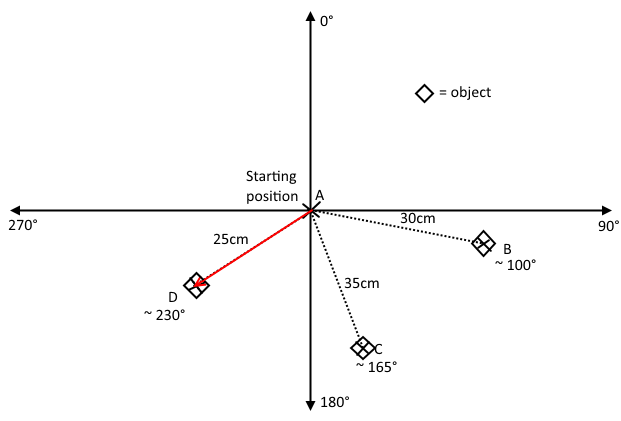
\includegraphics[width=\textwidth]
     {graphics/objectnavigationfirst.png}}}
     \caption{\label{fig:object_navigation_first} First object to be collected.}
\end{figure}

Now that the first object has been scheduled to be collected, the calculations uses trigonometry to find the shortest distance to the next object, and the angles that needs to be turned to face the starting position again. To increase the understanding, the state of the world is represented in \figref{fig:object_navigation_iteration}, where the actions to collect the first object has been applied and reflected in the figure. From this point, the distance to the remaining objects is calculated, using the formula:

\begin{equation}
a = \sqrt{ b^2 + c^2 - 2*b*c*cos(A) } \label{equation:a}
\end{equation}

But for this, the A angle is needed. This is calculated from the spotted angles during the search. The formula for calculating A is:

\begin{equation}
A = (Object~currently~at~spotted~angle) - (Object~closest~spotted~angle) \label{equation:AAngle}
\end{equation}

With the same method as the first object, the object with the shortest distance, from the current object, is found and saves the object number. Now the heading to the closest object must be calculated, and this is the angle calculated by the formula:

\begin{equation}
B = cos^{-1}((a^2 + c^2 - b^2)/(2*a*c)) \label{equation:B}
\end{equation}

This provides the angle that must be turned in order to face the next object. In \figref{fig:object_navigation_iteration} the \projname{} is pointed towards the starting position, and the angle that must be turned is calculated from equation \ref{equation:B}. The current heading added with the angle provides the heading to the next object. This angle is added to the instructions along with the distance. Then the final angle of the triangle is calculated, which is used to turn the \projname{} at the starting position again. The final angle is calculated with the formula:

\begin{equation}
C = 180 - A - B \label{equation:C}
\end{equation}

In order to point the \projname{} at the starting position again, the current heading is subtracted with (180 - C), where C is found by equation \ref{equation:C}. This process has provided the route to the next object, and the instructions to turn the \projname{} back, facing the starting position. The second step is executed for the remaining objects that were spotted. 

\begin{figure}[H]
     \center{\frame{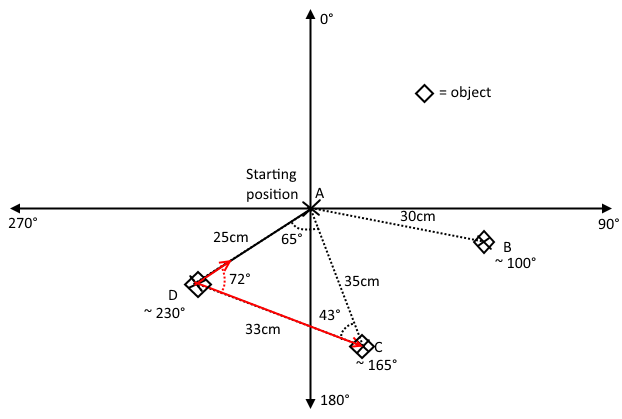
\includegraphics[width=\textwidth]
     {graphics/objectnavigationiteration.png}}}
     \caption{\label{fig:object_navigation_iteration} Iteration of objects to be collected.}
\end{figure}



%
% COMMENT
%
%\begin{comment}
\subsubsection*{Object navigation - implemented} \label{sec:objnav-implemented}

\lstref{lst:objectnavigation1} and \lstref{lst:objectnavigation2} shows the algorithm, as tried to implemented in the \projname{}. It practically works the same way as the concept, but with a few adjustments to make it work. An important little workaround is the boolean \emph{flipped} variable. This is used to decide to which direction, the \projname{} should turn, in order to get to the next object. The problem with choosing the direction is sketched in \figref{fig:choosingdirection}, to help understanding. The difference in angles is calculated, from the object where the \projname{} is currently at. Then angle is checked using the \emph{CalculateValidAngle} function, that ensures that the value is within the possible values (0 - 359). If the difference in angle is bigger than 180, then the flipped variable is set to true, meaning that the turning direction is left, else turn to the right. The \emph{flipped divider}, from \figref{fig:choosingdirection}, shows to which side the \projname{} should turn, depending on which side the object is located. Depending on which side the object is located, different measures to find the angle is used, as shown on in \figref{fig:choosingdirection} This provides us with the correct angle, that should be turned to face the next object. 

\begin{figure}[H]
     \center{\frame{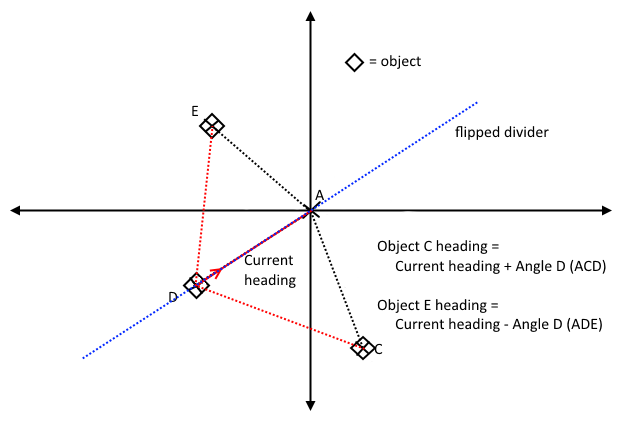
\includegraphics[width=\textwidth]
     {graphics/objnavchoosingdirection.png}}}
     \caption{\label{fig:choosingdirection} Choosing the direction.}
\end{figure}

The algorithm used a boolean array to control which object it has collected, ensuring that the object is removed from the remaining objects, as the \projname{} should only get to each object once. 

The first part of the algorithm can be seen in \lstref{lst:objectnavigation1}. This part shows the initialisation of variables and the input parameters. At line 19, the helper function \emph{FindClosestObjects} is used to find the closest object. Then the case for the first object is shown, where no trigonometry is needed to calculate, as this is from the starting position, knowledge about angle and distance is known from the sensors. 

\begin{lstlisting}[caption= Object navigation start and for the first object, label=lst:objectnavigation1]
void ObjectNavigation(OBJECT objects[], int objectsFound, OBJECT instructions[], OBJECT turnToStartInstructions[])
{
	int addedToRoute = 0;
	int previousObjectNumber = 0;
	int closestObjectNumber = 0;
	S16 currentHeading = compass.getHeading(); 
	bool hasBeenAdded[objectsFound];
	bool flipped = false; 
	
	for (int j = 0; j <= objectsFound; j++)
	{
		flipped = false; 
		closestObjectNumber = findClosestObjects(objects, objectsFound, addedToRoute, previousObjectNumber,  hasBeenAdded);
		
		if (j == 0)
		{
			instructions[j].angle = objects[closestObjectNumber].angle;
			currentHeading = objects[closestObjectNumber].angle;
			instructions[j].distance = objects[closestObjectNumber].distance;
			hasBeenAdded[closestObjectNumber] = true;
			
			previousObjectNumber = closestObjectNumber;
			turnToStartInstructions[j].angle = CalculateValidAngle(currentHeading, 180);
			currentHeading = turnToStartInstructions[j].angle;
			addedToRoute++;
		}
\end{lstlisting}

\lstref{lst:objectnavigation2} shows the case for the n'th object. The difference here is the use of trigonometry to calculate the next angle to turn and distance to travel. Mathematical concepts presented in \secref{sec:objnav-concept} is used to calculate the angles and distances. 

\begin{lstlisting}[caption= Object navigation n'th object, label=lst:objectnavigation2]
		else if (j > 0)
		{
			int b = objects[closestObjectNumber].distance;	
			int c = objects[previousObjectNumber].distance;
			int aAngle = CalculateValidAngle(objects[previousObjectNumber].angle, -objects[closestObjectNumber].angle);
			if (180 < aAngle && aAngle <= 359)
			{
				flipped = true;
			}
			int a = static_cast<int>(sqrt(pow(b, 2)+pow(c, 2)-2*b*c*cos((aAngle*PI)/180)));
			int bAngle = static_cast<int>(acos((pow(a, 2)+pow(c, 2)-pow(b, 2))/(2*a*c)) * 180 / PI);
			int cAngle = ((180 - aAngle) - bAngle);

			instructions[j].angle = (flipped == false) ? (currentHeading+bAngle) : (currentHeading-bAngle);
			instructions[j].distance = a;
			hasBeenAdded[closestObjectNumber] = true; 
			previousObjectNumber = closestObjectNumber;
			turnToStartInstructions[j].angle = (flipped == false) ? CalculateValidAngle(currentHeading, (180-cAngle)) : CalculateValidAngle(currentHeading, -(180-cAngle));
			currentHeading = turnToStartInstructions[j].angle;
			addedToRoute++;
		}
	}
}
\end{lstlisting}


The algorithm uses a function to help find the closest object. This is used to divide the task to increase readability. The \emph{FindClosestObject}, seen in \lstref{lst:findclosestobject}, takes all the objects as input, an array to check which object has been added and knowledge about the last object that was chosen. From this, it checks the objects, those that has not already been added, from the last objects location. The last objects location is the starting position for the first object. The distance to all the other remaining objects is then calculated and the object closest is chosen and returned. 

\begin{lstlisting}[caption= Function findClosestObject, label=lst:findclosestobject]
int FindClosestObjects(OBJECT objects[], int objectsFound, int addedToRoute, int previousObjectNumber, bool hasBeenAdded[])
{
	int closestObjectNumber = -1; 
	int tempDistance = 2000; 
	
	for (int i = 0; i <= objectsFound; i++)
	{
		if (addedToRoute == 0)
		{
			if (objects[i].distance < tempDistance)
			{
				tempDistance = objects[i].distance;
				closestObjectNumber = i;
			}
		}
		
		else if (addedToRoute > 0 && hasBeenAdded[i] == false)
		{
			int b = objects[i].distance;
			int c = objects[previousObjectNumber].distance;
			int aAngle = objects[previousObjectNumber].angle - objects[i].angle;
			if ( aAngle < 0 )
			{
				aAngle = -aAngle;
			}
			int a = static_cast<int>(sqrt(pow(b, 2)-pow(c, 2)-2*b*c*cos((aAngle*PI)/180)));
			
			if ( a < tempDistance )
			{
				tempDistance = a;
				closestObjectNumber = i;
			}
		}
	}
	return closestObjectNumber;
}
\end{lstlisting}

Despite several tests and number tweaking within the algorithm, the problems with the ultrasonic sensor, see \secref{sec:ultrasonic_sensor}, were too severe to get the initial search to work. The sensor were not able to spot the right amount of objects and the precision of the objects were not correct, which resulted in a calculated route that would not hit the objects. It was therefore decided to use the next-in-view algorithm as described in the sixth iteration in \secref{sec:imp-procedure}.
\end{comment}
%
% COMMENT
%
%%The motor controller is split up into two parts: one part for rotation and one part for moving forward and backward. Both part have a function for adjusting the speed and stop the motors on the target angle or step. Only the code for the moving forward and backwards is include in this section, as the code only has small differences.

%The code in \lstref{lst:speed-adjuster1of2} shows the first part of the function to adjust the speed when the robot is moving forward and backwards. This part calculates the min and max steps, that both motors has to be inside. The if-else check ensures that the speed is not set too low or high, else provides a minimum or maximum value for the motors. 

%The second part of the speed adjust code is shown in \lstref{lst:speed-adjuster2of2}. Line 1 checks if the current number of steps for the left motor is inside the min/max range. If that is the case, then the speed adjuster does nothing, and returns the current speed. If the amount of steps is outside the min/max range, line 5 and 16 checks whether the speed should be increased or decreased. 

%\lstref{lst:motor-controller} shows the function to check whether or not the \projname{} has reached the targeted amount of steps. Line 9 and 14 checks which way the \projname{} must move in order to reach the target. If the target is reached the else at line 19 stops the motors.


% Algorithm description
%\subsection{Algorithm description} \label{sec:algorithm-desc}

After the \projname{} has completed its initial 360 degree search and stored the information about the nearby objects, it is time to calculate a route between said objects. Due to the limited power and calculation speed of the LEGO NXT brick it is necessary to find an efficient algorithm that is fast and does not take a lot of computational power and space. 

The shortest route between the object can be brute forced by trying out every single possible route between the start position and all of the objects. This would have a calculation time of $\mathcal{O}(n!)$, which means that every object added greatly increases the running time. This gives the robot problems when calculating a shortest route, if the amount of objects exceed a certain number. If there are 9 objects, the number of different paths to check exceeds 360000. 

A more time efficient, but less effective, algorithm is the NN-algorithm. The algorithm calculates a route based on which objects are closest together. This means that the distance to all the points are calculated from the starting point and the shortest distance is chosen. This is then repeated from the new point, but this time it does not calculate from any previously visited points.

A very simple algorithm, that uses very little calculation, is the next-in-view algorithm. This was the first algorithm to be implemented on the \projname{} due to its simplicity. With this algorithm, the robot starts turning towards either right or left, stopping at the first object it detects. It then moves out to collect this object, and then starts turning towards the same direction again, thus always picking up the next object that comes into its view, hence the name of the algorithm. This algorithm has a number of issues connected to it, which may reduce its performance, however in smaller cases with less than ten objects, its completion speed is close to the NN-algorithm.

\begin{figure}[H]
     \center\frame{{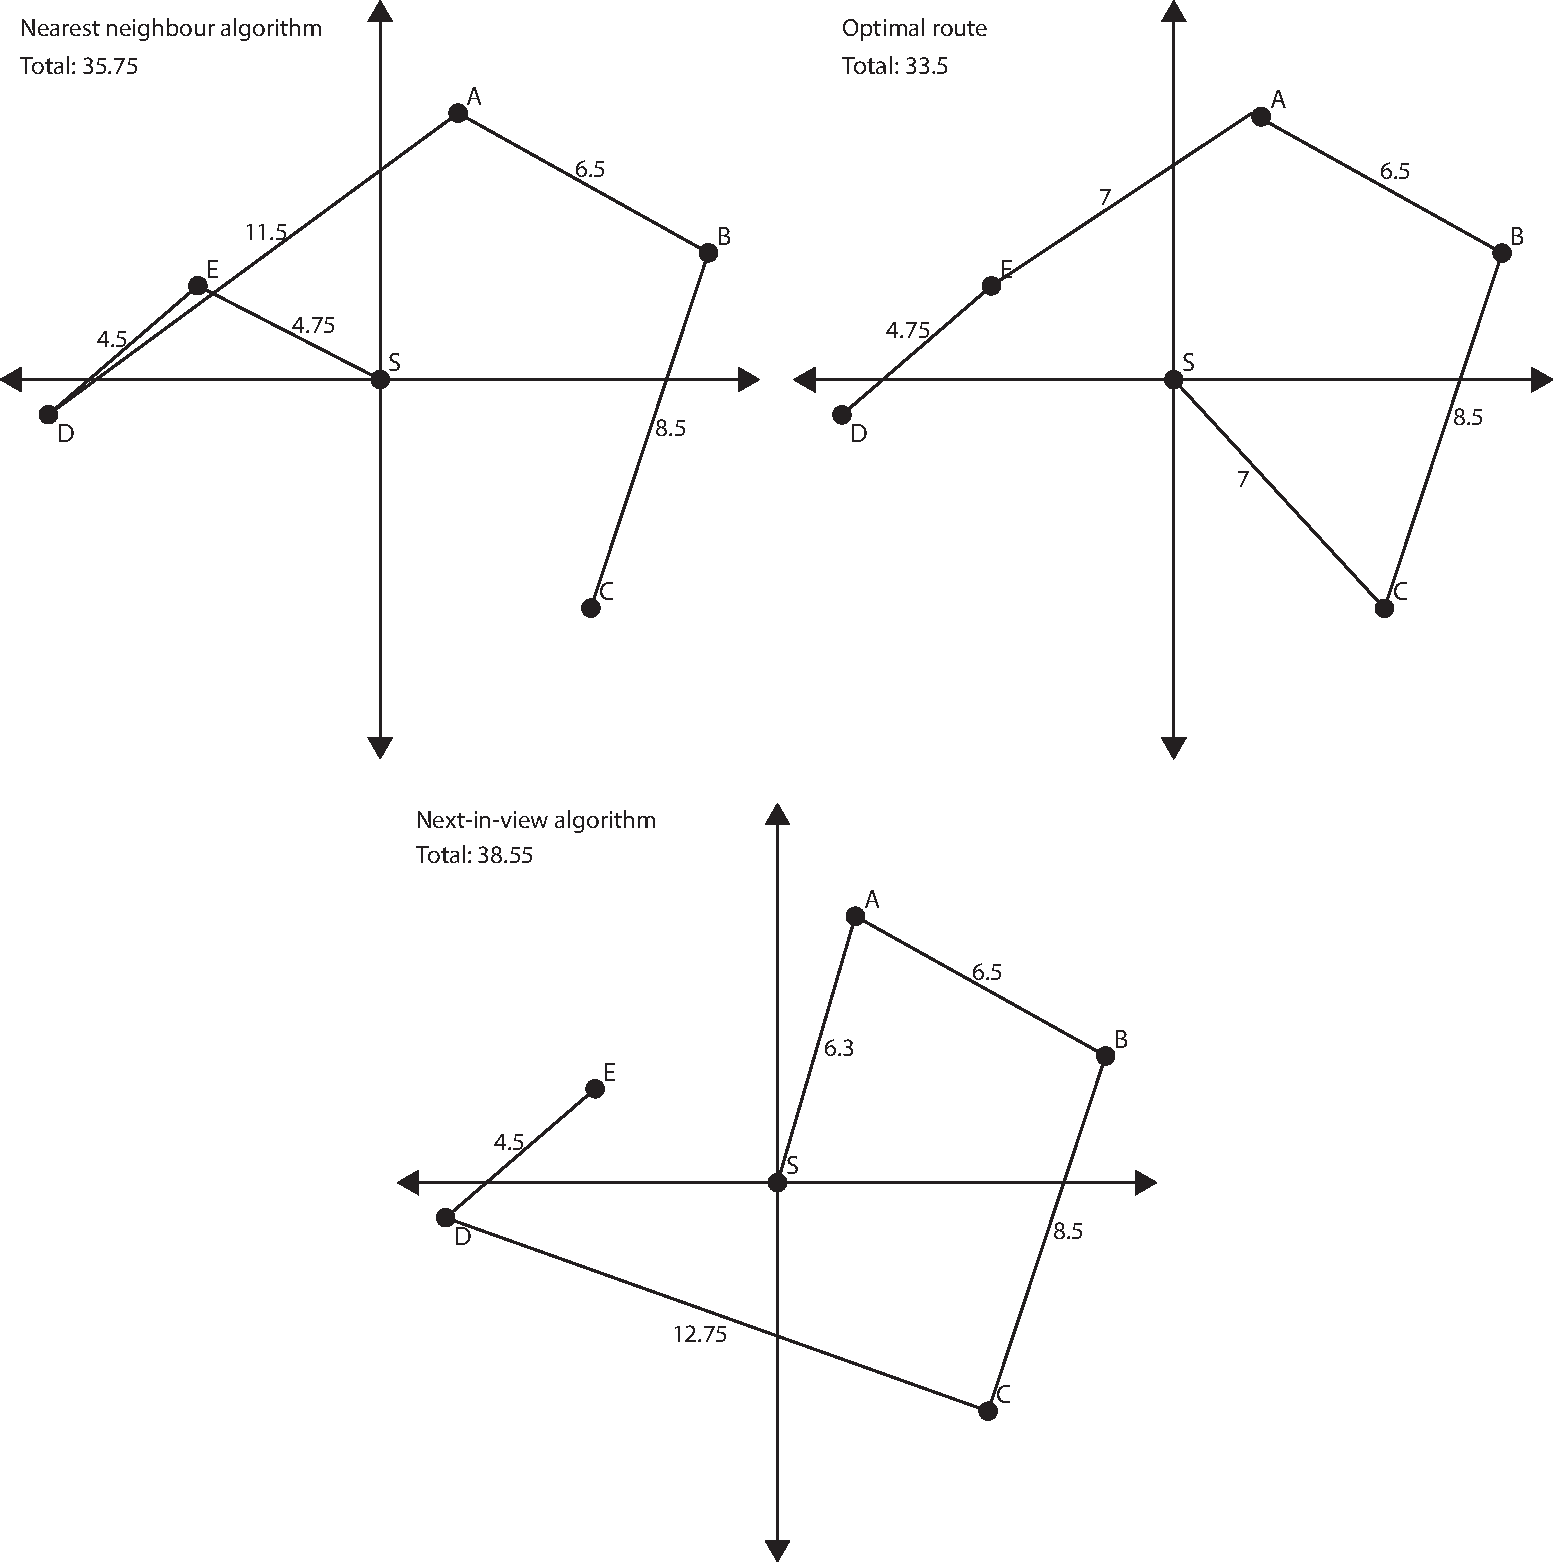
\includegraphics[width=\textwidth]
     {graphics/AlgorithmExamples2.pdf}}}
     \caption{\label{fig:algorithm-example} Example of the NN-algorithm, the optimal algorithm, and next-in-view algorithms.}
\end{figure}

\figref{fig:algorithm-example} shows three solutions to the problem. The top right graph is the optimal solution, which is only used to compare the results from the two other algorithms. Top left is the NN-algorithm, and in the bottom the next-in-view algorithm. The robot starts its route at position \emph{S}. The objects are named in order as they are first detected. The algorithms result in the routes shown on the figure.

The different solutions in \figref{fig:algorithm-example} have following lengths:
\begin{itemize}
\item Optimal: 33.5 units
\item NN-algorithm: 35.75 units
\item Next-in-view: 38.55 units
\end{itemize}

In the average case, the difference between the NN-algorithm and the next-in-view solutions would be larger if there were more objects to consider. However for these smaller cases, the difference is almost negligible. It should be noted, that this does not describe the time spent, only the distance travelled: rotation to scan for objects, for both algorithms, will also take different amounts of time depending on the case. This is not accounted for here.

Due to the limitations of the LEGO NXT brick and the complexity of the problem, finding the optimal solution was ruled out as a possibility. Instead, the NN-algorithm was initially selected to calculate the route for the \projname{}. This algorithm does not always result in the most optimal route, but when the calculation speed and actual running speed is considered, it is arguably faster in the average case. However, as previously mentioned, this algorithm was not implemented. This was the result of inaccurate hardware: the ultrasonic sensor was not able to detect objects with enough precision, that the \projname{} could accurately calculate any useful information based on the data.

Due to this limitation, the \emph{next-in-view} algorithm was chosen for implementation. The simplicity of the algorithm, as well as the fact that it takes the inaccurate sensor input into account, made it the obvious choice. And as previously mentioned in \secref{sec:nn-algorithm}, the distance difference of the two algorithms are nearly insignificant.

